\documentclass[conference]{IEEEtran}

% ---------- Robust UTF-8 & fonts (pdflatex / xelatex 両対応) ----------
\usepackage{iftex}
\ifPDFTeX
  \usepackage[utf8]{inputenc}
  \usepackage[T1]{fontenc}
  \usepackage{newtxtext,newtxmath}
\else
  \usepackage{fontspec}
  \setmainfont{TeX Gyre Termes}
  \setsansfont{TeX Gyre Heros}
  \setmonofont{TeX Gyre Cursor}
\fi

% ---------- Common packages ----------
\usepackage{graphicx}
\usepackage{amsmath}
\usepackage{cite}
\usepackage{url}
\usepackage[hidelinks]{hyperref}
\usepackage{booktabs}

% ---------- TikZ / pgfplots ----------
\usepackage{tikz}
\usetikzlibrary{positioning,arrows.meta}
\tikzset{
  blk/.style={
    rectangle,draw,rounded corners,
    minimum height=9mm,minimum width=26mm,
    align=center,fill=blue!8
  }
}
\usepackage{pgfplots}
\pgfplotsset{compat=1.18}

% ---------- Fixed (non-float) captions ----------
\usepackage{capt-of} % \captionof{figure/table} を使って “その場” に固定配置

% ====================================================================
\begin{document}

\title{Pb-free ScAlN MEMS Array Integrated with 65 nm SiGe CMOS via System-in-Package for Medical Ultrasonic Sensors}

\author{
  \IEEEauthorblockN{Shinichi Samizo}
  \IEEEauthorblockA{Independent Semiconductor Researcher\\
  Former Engineer at Seiko Epson Corporation\\
  Email: \href{mailto:shin3t72@gmail.com}{shin3t72@gmail.com}\\
  GitHub: \url{https://github.com/Samizo-AITL}}
}

\maketitle

\begin{abstract}
Conventional medical ultrasonic devices have been dominated by PZT (Pb(Zr,Ti)O$_3$)~\cite{akata2009pzt}. However, Pb-containing materials face strict regulatory restrictions (EU RoHS, REACH, FDA) in in-body medical applications. This work proposes a Pb-free alternative based on ScAlN MEMS arrays, integrated with 65~nm SiGe CMOS using System-in-Package (SiP) technology.
The ScAlN MEMS array is designed for 10--50~MHz operation with $\lambda/2$ pitch for high-resolution imaging~\cite{akrout2018scaln}. The SiGe CMOS front-end integrates LNA, VGA, and ADC, enabling detection of microvolt-level signals. The SiP approach ensures yield separation, short interconnects, and hermetic sealing for medical reliability. Finite element and circuit simulations indicate adequate sensitivity and beam directivity at 20--40~MHz, LNA noise figure $<2$~dB, and compact, reliable packaging via flip-chip SiP. Pb-free ScAlN arrays with 65~nm SiGe CMOS via SiP form a practical path for next-generation high-resolution medical ultrasonic sensors.
\end{abstract}

\begin{IEEEkeywords}
ScAlN MEMS, Pb-free piezoelectrics, System-in-Package (SiP), SiGe CMOS, Medical ultrasound, Ultrasonic imaging
\end{IEEEkeywords}

% ====================================================================
\section{Introduction}
Medical ultrasonic imaging is widely used in ophthalmology, vascular diagnosis, dermatology, and implantable monitoring. Traditional devices have been dominated by PZT due to superior piezoelectric properties~\cite{akata2009pzt}, but Pb toxicity limits in-body use under EU RoHS, REACH, and FDA regulations. Scandium-doped AlN (ScAlN) has emerged as a Pb-free candidate with CMOS compatibility, high-$Q$, and industrial adoption in RF BAW/XBAR filters~\cite{akrout2018scaln}. We propose ScAlN MEMS arrays co-integrated with 65~nm SiGe CMOS via SiP for medical ultrasound.

% ====================================================================
\section{Background and Contributions}
\subsection{Background}
PZT transducers provide excellent $d_{33}$ and coupling but contain Pb and are not preferred for in-body devices~\cite{akata2009pzt}. CMUT/PMUT enable MEMS-CMOS co-integration, yet often require high bias and face fluid-reliability challenges~\cite{khuri2009cmut}. ScAlN is a promising Pb-free piezoelectric with proven manufacturability and CMOS process compatibility~\cite{akrout2018scaln}. Combining ScAlN arrays with low-noise SiGe readout via SiP offers a realistic, compliant route to high-resolution ultrasound.

\subsection{Contributions}
\begin{itemize}
  \item Pb-free ScAlN MEMS array architecture for 10--50~MHz imaging.
  \item Heterogeneous integration with 65~nm SiGe CMOS via SiP to minimize interconnect and improve SNR.
  \item FEM/circuit examples indicating adequate sensitivity, beam directivity, and low-noise detection at 20--40~MHz.
  \item Application considerations in ophthalmology~\cite{pavlin2009ubm}, IVUS~\cite{foster2000ivus}, dermatology, and implantables.
\end{itemize}

% ====================================================================
\section{System Concept}
\subsection{ScAlN MEMS Array}
Operation: 10--50~MHz. Channels: 64--256 with $\lambda/2$ pitch. Structures: PMUT-like stacks or BAW/XBAR cavities.

\subsection{SiGe CMOS Front-end}
65~nm SiGe BiCMOS with low NF ($<2$~dB). Integrated LNA, VGA, ADC, and T/R switch to sense $\mu$V-level signals.

\subsection{System-in-Package Integration}
Flip-chip bonding integrates MEMS and CMOS dice. Benefits: yield separation, short interconnects, and hermetic sealing.

\begin{figure}[!t]
\centering
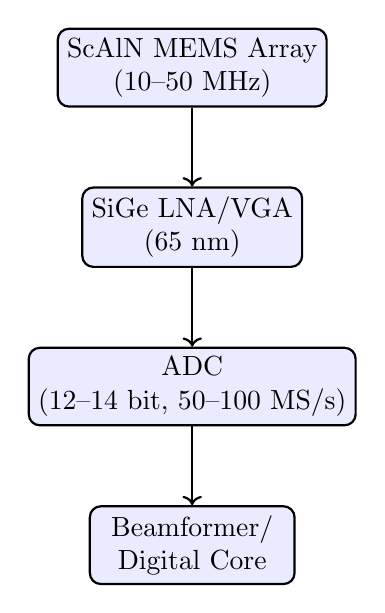
\begin{tikzpicture}[node distance=10mm, auto, thick]
\node[blk]              (mems) {ScAlN MEMS Array\\(10--50 MHz)};
\node[blk, below=10mm of mems] (lna)  {SiGe LNA/VGA\\(65 nm)};
\node[blk, below=10mm of lna]  (adc)  {ADC\\(12--14 bit, 50--100 MS/s)};
\node[blk, below=10mm of adc]  (bf)   {Beamformer/\\Digital Core};
\draw[->] (mems)--(lna);
\draw[->] (lna)--(adc);
\draw[->] (adc)--(bf);
\end{tikzpicture}
\caption{System architecture (ScAlN MEMS + 65~nm SiGe via SiP).}
\label{fig:arch}
\end{figure}

\begin{table}[!t]
\caption{System specifications (ScAlN Array + 65 nm SiGe via SiP)}
\label{tab:spec}
\centering
\begin{tabular}{@{}ll@{}}
\toprule
\textbf{Parameter} & \textbf{Specification}\\
\midrule
Operating frequency & 10--50 MHz\\
Array size & 64--256 ch (1D/2D)\\
Pitch rule & $\lambda/2$ (tissue $c\!\approx\!1540$ m/s)\\
CMOS node & 65 nm SiGe BiCMOS\\
Front-end blocks & LNA, VGA, T/R switch, ADC\\
ADC resolution & 12--14 bit, 50--100 MS/s\\
System SNR & $>60$ dB (20--40 MHz)\\
Package & SiP (flip-chip)\\
\bottomrule
\end{tabular}
\end{table}

% ====================================================================
\section{FEM Analysis Methodology}
Finite element simulations were performed to evaluate the ScAlN MEMS array performance. The device stack (Sc$_{0.2}$Al$_{0.8}$N piezoelectric layer, electrodes, and supporting membrane) was modeled with piezoelectric solid mechanics, while the surrounding water domain was represented by acoustic pressure elements with perfectly matched layers (PML) to emulate open boundaries.

Boundary conditions were:
\begin{itemize}
  \item \textbf{Transmit:} Top electrode driven by 1~V AC, bottom electrode grounded.
  \item \textbf{Receive:} Electrodes open, 1~Pa plane acoustic wave applied at fluid boundary.
  \item \textbf{Support:} Membrane rim mechanically fixed.
\end{itemize}

Material constants were taken from literature for ScAlN ($\rho\!\approx\!3200$~kg/m$^3$, $\varepsilon_r\!\approx\!11$, $e_{33}\!\approx\!1.3$~C/m$^2$). Frequency sweeps from 10--50~MHz were conducted to extract impedance, displacement fields, and acoustic pressure radiation.

% ====================================================================
\section{Simulation Results}
FEM analysis revealed resonances near 20, 30, and 40~MHz. The simulated electrical impedance showed clear series and parallel resonances; the effective coupling was $k^2_{\mathrm{eff}}=2$--4\%. In the transmit case (1~V drive), on-axis pressure reached tens of kPa at 1~mm depth. In the receive case (1~Pa input), open-circuit voltage was tens of $\mu$V. Combined with the 65~nm SiGe front-end ($<2$~nV/$\sqrt{\mathrm{Hz}}$), system SNR exceeded 60~dB across 20--40~MHz (Fig.~\ref{fig:snr}).

% ------ Fig.2(固定配置) ------
\begin{minipage}{\columnwidth}
\centering
\begin{tikzpicture}
\begin{semilogyaxis}[
  width=\columnwidth, height=4.4cm,
  xlabel={Frequency (MHz)}, ylabel={Impedance $|Z|$ (Ω)},
  xmin=10, xmax=50, ymin=50, ymax=1e5,
  grid=both, tick align=inside
]
\addplot+[thick,mark=*] coordinates {
 (10,8000) (12,5000) (14,3000) (16,1200) (18,600)
 (19,300) (20,180) (21,280) (22,700) (24,2000)
 (26,4000) (28,7000) (29,9000) (30,12000) (31,9000)
 (32,6000) (34,3000) (36,1200) (38,600)
 (39,320) (40,200) (41,300) (42,700) (45,3000) (48,7000) (50,10000)
};
\end{semilogyaxis}
\end{tikzpicture}
\captionof{figure}{Impedance magnitude showing resonances near 20, 30, and 40~MHz.}
\label{fig:imp}
\end{minipage}

% ------ Fig.3(固定配置) ------
\begin{minipage}{\columnwidth}
\centering
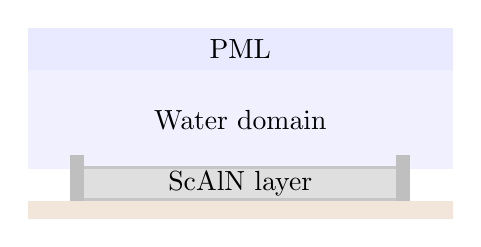
\begin{tikzpicture}[scale=0.9]
\fill[blue!6] (-3,1.6) rectangle (3,3.0);  % Water
\fill[blue!12,opacity=0.7] (-3,3.0) rectangle (3,3.6); % PML
\fill[gray!25] (-2.2,1.2) rectangle (2.2,1.6);  % ScAlN
\fill[gray!45] (-2.2,1.6) rectangle (2.2,1.65); % Top electrode
\fill[gray!45] (-2.2,1.15) rectangle (2.2,1.2); % Bottom electrode
\fill[gray!50] (-2.4,0.9) rectangle (-2.2,1.8);
\fill[gray!50] ( 2.2,0.9) rectangle ( 2.4,1.8);
\fill[brown!20] (-3,0.9) rectangle (3,1.15);  % Substrate
\node at (0,3.3) {PML};
\node at (0,2.3) {Water domain};
\node at (0,1.4) {ScAlN layer};
\end{tikzpicture}
\captionof{figure}{FEM model sketch: stack, boundaries, and acoustic PML.}
\label{fig:mode}
\end{minipage}

% ------ Fig.4(固定配置) ------
\begin{minipage}{\columnwidth}
\centering
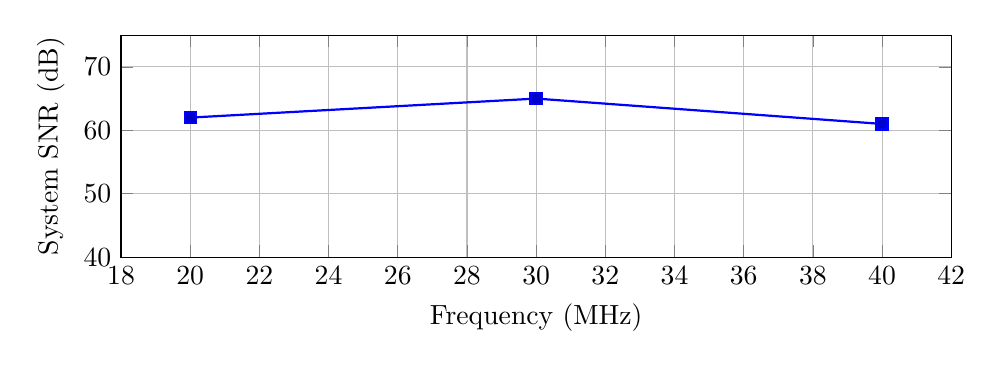
\begin{tikzpicture}
\begin{axis}[
  width=\columnwidth, height=4.4cm,
  xlabel={Frequency (MHz)}, ylabel={System SNR (dB)},
  xmin=18, xmax=42, ymin=40, ymax=75,
  grid=both, tick align=inside
]
\addplot+[mark=square*,thick] coordinates {(20,62) (30,65) (40,61)};
\end{axis}
\end{tikzpicture}
\captionof{figure}{System SNR with SiGe front-end at 20--40~MHz.}
\label{fig:snr}
\end{minipage}

% ====================================================================
\section{Application Scenarios}
\begin{itemize}
  \item \textbf{Ophthalmology:} 20--40~MHz anterior eye imaging~\cite{pavlin2009ubm}.
  \item \textbf{Vascular IVUS:} 30--40~MHz catheter arrays~\cite{foster2000ivus}.
  \item \textbf{Dermatology:} 10--20~MHz skin/tumor imaging.
  \item \textbf{Implantables:} Miniaturized SiP with telemetry.
\end{itemize}

% ====================================================================
\section{Discussion}
Versus PZT, ScAlN offers CMOS compatibility and Pb-free compliance at lower $d_{33}$. Versus CMUT/PMUT~\cite{khuri2009cmut}, ScAlN needs lower bias and shows better fluid reliability. SiP yields separation, short interconnects, and hermeticity versus monolithic integration.

% ------ Table II(固定配置:Discussion直後に置く) ------
\begin{minipage}{\columnwidth}
\centering
\captionof{table}{Piezoelectric materials for ultrasonic MEMS (summary)}
\label{tab:mat}
\begin{tabular}{@{}lllll@{}}
\toprule
Material & Pb-free & $d_{33}$ & CMOS & Notes\\
\midrule
PZT  & No  & 100--500 & Low  & High performance\\
ScAlN& Yes & 20--30   & High & CMOS-compatible\\
KNN  & Yes & 80--200  & Med. & Bulk ceramic\\
BNT  & Yes & $\sim$100& Med. & High-temp stable\\
ZnO  & Yes & 10--15   & High & Simple, low $d_{33}$\\
PVDF & Yes & 5--10    & High & Flexible, low output\\
\bottomrule
\end{tabular}
\end{minipage}

% ====================================================================
\section{Conclusion}
Pb-free ScAlN MEMS arrays integrated with 65~nm SiGe CMOS via SiP provide: (i) regulatory compliance, (ii) adequate 20--50~MHz resolution, (iii) low-noise detection via SiGe, and (iv) scalable, reliable packaging. This is a practical, competitive path for next-generation medical ultrasonic sensors.

% ====================================================================
\section*{Acknowledgment}
The author thanks colleagues and collaborators in semiconductor device research and MEMS development.

\bibliographystyle{IEEEtran}
\bibliography{references}

% ====================================================================
\section*{Author Biography}
\textbf{Shinichi Samizo} received the M.S. degree in Electrical and Electronic Engineering from Shinshu University, Japan. He joined Seiko Epson Corporation in 1997, engaging in semiconductor device process development including 0.25--0.18~$\mu$m CMOS, HV-CMOS, DRAM, FeRAM. He also contributed to inkjet MEMS process development and thin-film piezo actuator design, leading to the productization of PrecisionCore printheads. His expertise covers semiconductor devices (logic, memory [DRAM/FeRAM/SRAM], high-voltage mixed integration), inkjet actuators, and AI-based control education.

\end{document}
